\documentclass{beamer}
\usepackage{pgf}
\usepackage{polski}
\usepackage[polish]{babel}
\usepackage[utf8]{inputenc}
\usepackage{xcolor}
\usepackage{graphicx}
\usepackage{array,makecell}
\graphicspath{{Grafiki/}}
\usetheme{Singapore}
\usecolortheme{seagull}
\setbeamertemplate{navigation symbols}{}

\title{Wykorzystanie sieci neuronowych i algorytmu najbliższych sąsiadów do implementacji wirtualnego sensora temperatury zapłonu kerozyny}
\author{Łukasz Meyer\\  Arkadiusz Piórkowski}

\begin{document}
\begin{frame}
	\titlepage
\end{frame}

\begin{frame}{Ścieżka prowadzenia projektu}
\begin{enumerate}
	\item Przegląd literatury
	\item Wstępna ocena danych (wizualna, współczynnik $R^2$)
	\item Opracowanie modelu opartego o sieć neuronową
	\item Testy i optymalizacja sieci neuronowej
	\item Opracowanie modelu opartego o algorytm k-NN
	\item Testy i dobór parametrów modelu k-NN
	\item Porównanie modeli, wyznaczenie średniej z dwóch modeli
\end{enumerate}
\end{frame}

\begin{frame}{Przegląd literatury}
\begin{columns}
\column{0.7\textwidth}
\begin{figure}
	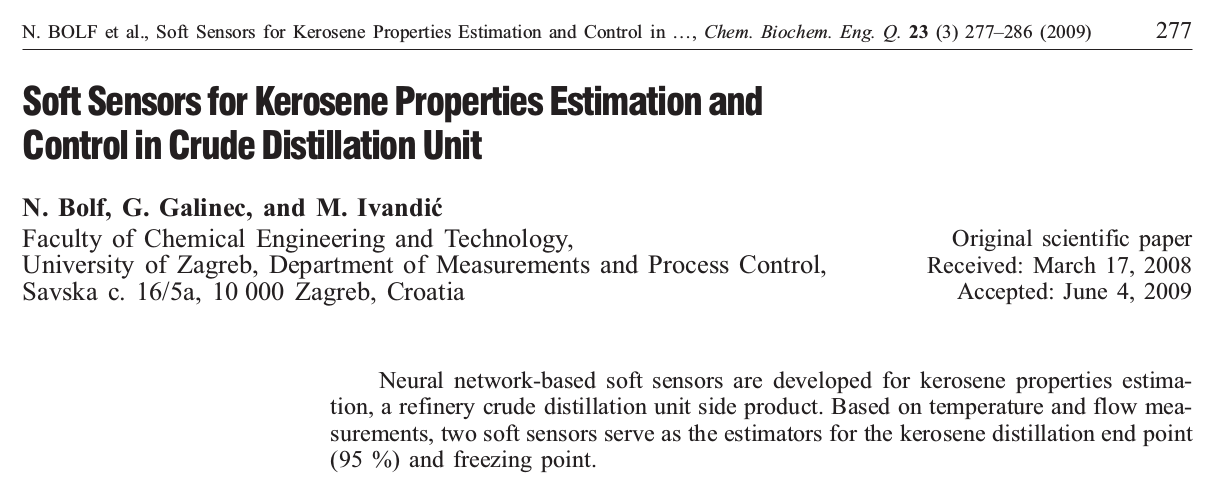
\includegraphics[width=\linewidth]{cabeq_1}
\end{figure}
%\begin{figure}
%	
\includegraphics[width=\linewidth]{crudeUnit_nn_abb}
%\end{figure}
\column{0.3\textwidth}
\begin{figure}
	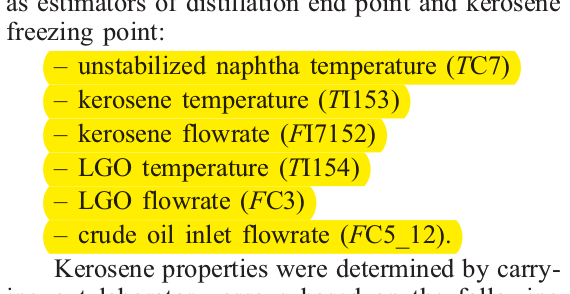
\includegraphics[width=\linewidth]{cabeq_2}
\end{figure}
\end{columns}

\end{frame}

\begin{frame}{Wstępna analiza danych}
\begin{columns}
\column{0.4\textwidth}
\begin{table}[ht]
	\begin{tabular}{|c|c|}
 		\hline
		Parametr & $R^2$ \\
		\hline
		FC0206 & $0.416$ \\
		\hline
		TI0208 & $0.411$ \\
		\hline
		TI0240 & $0.409$\\
		\hline
		TI0265 & $0.363$\\
		\hline
 		FC0211 & $0.353$\\
		\hline
		TI0206 & $0.339$\\
		\hline
		TI0204 & $0.306$\\
		\hline
		TI0250 & $0.295$\\
		\hline
		TI0278 & $0.162$\\
		\hline
	\end{tabular}
	\caption{Dopasowanie do prostej, uśrednianie wejść z 5 godzin przed pomiarem $T_{A22}$}
\end{table}
\column{0.7\textwidth}
\begin{figure}
	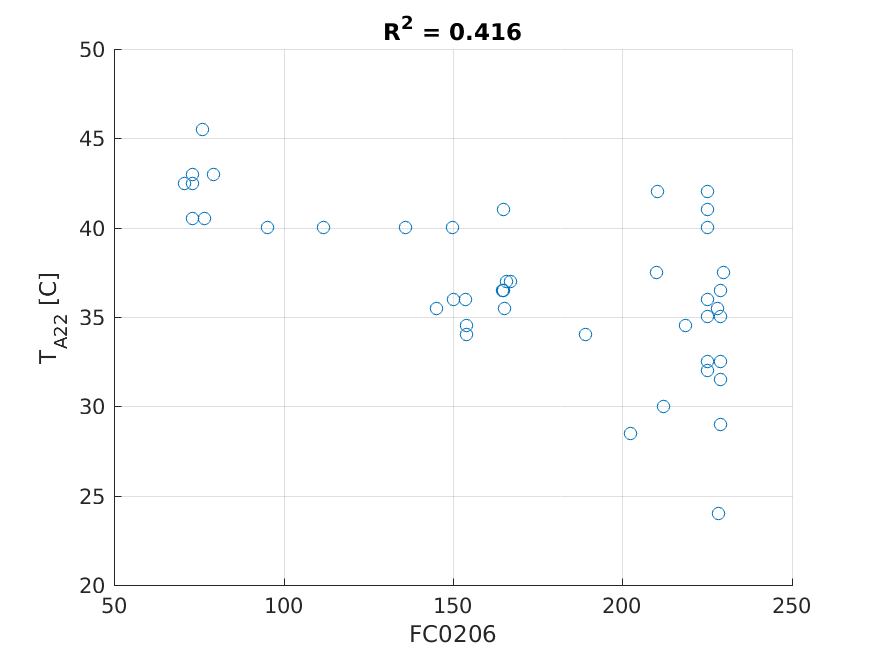
\includegraphics[width=\linewidth]{FC0206}
\end{figure}
\end{columns}
\end{frame}

\begin{frame}{Sieć neuronowa - idea przyrostów od poprzedniego pomiaru}
\begin{figure}
	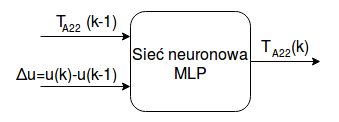
\includegraphics[width=\linewidth]{diagram_nn}
\end{figure}

%\begin{columns}
	%\column{0.6\textwidth}
	\begin{itemize}
		\item $T_{A22}(k-1)$- poprzedni pomiar laboratoryjny. Uwzględnia jakość ropy i jej skład. (założenie: jakość i parametry ropy nie zmieniają się drastycznie z tygodnia na tydzień).
		\item $\Delta u$ - przyrosty wejść (6 temperatur, 2 przepływy) względem chwili wykonania poprzedniego pomiaru laboratoryjnego
	\end{itemize}
	%\column{0.4\textwidth}
%\end{columns}

\end{frame}

\begin{frame}{Uczenie sieci}
Otrzymany zbiór danych uczących dzielony jest losowo na zbiory: uczący sieć i walidacyjny.
\begin{columns}
	\column{0.6\textwidth}
	\begin{figure}
		\centering
		\makebox[\textwidth][c]{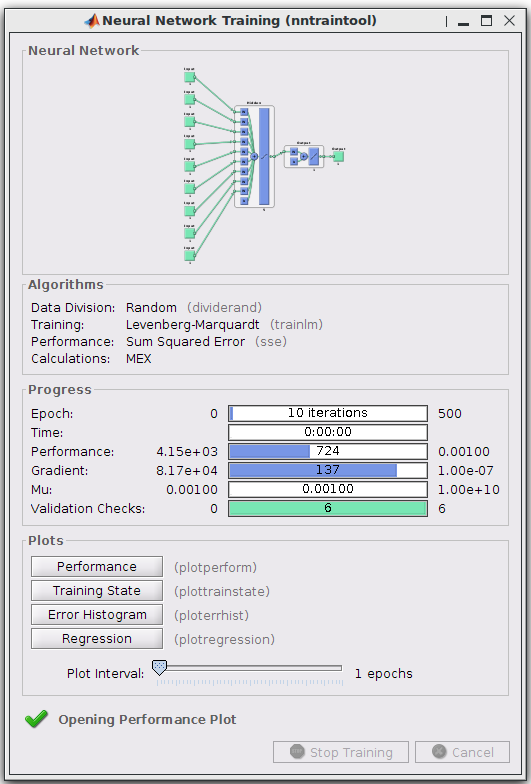
\includegraphics[width=0.5\textwidth]{nn_train_window}}
		\caption{Wykorzystano sieć \textit{feedforwardnet} i Neural Network Toolbox MATLABa}
	\end{figure}
	
	\column{0.4\textwidth}
	\begin{figure}
		\centering
		\makebox[\textwidth][c]{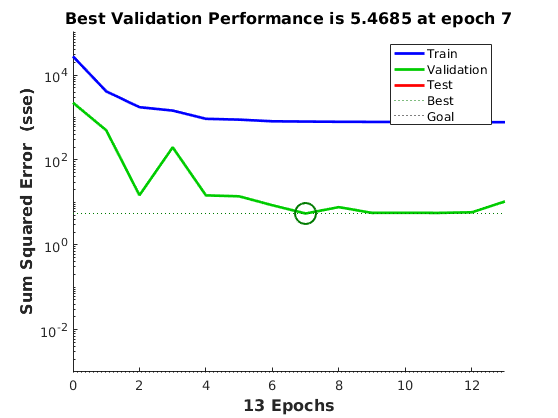
\includegraphics[width=1.2\textwidth]{nn_train_performance}}
		\caption{Przebieg błędu podczas uczenia sieci neuronowej}
	\end{figure}
\end{columns}
\end{frame}

\begin{frame}{Rezultaty}
\begin{columns}
	\column{0.5\textwidth}
	\begin{figure}
		\centering
		\makebox[\textwidth][c]{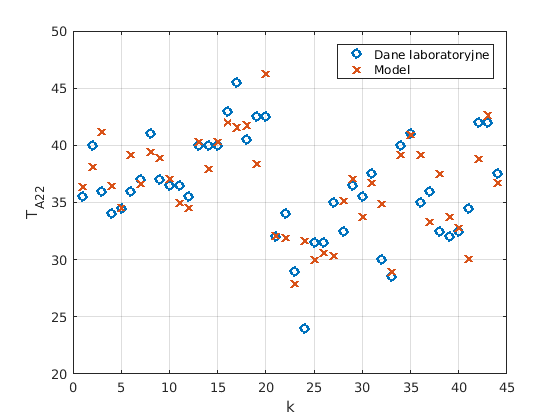
\includegraphics[width=1.2\textwidth]{proper_nn_train_1}}
		\caption{Działanie modelu dla danych uczących; $E=6.02\%$}
	\end{figure}
	
	\column{0.5\textwidth}
	\begin{figure}
		\centering
		\makebox[\textwidth][c]{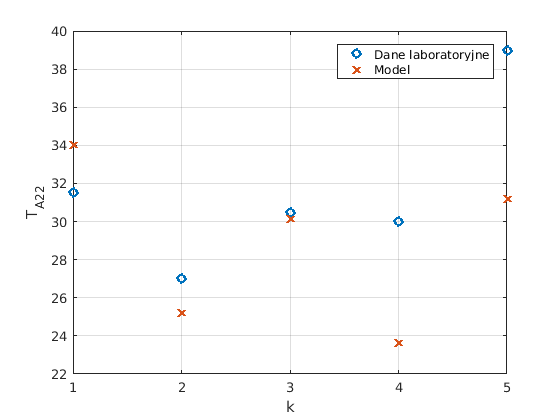
\includegraphics[width=1.2\textwidth]{proper_nn_valid_1}}
		\caption{Działanie modelu dla danych walidacyjnych(2); $E=9.2\%$}
	\end{figure}
\end{columns}
\end{frame}

\begin{frame}{Algorytm K-NN}
	\begin{figure}
		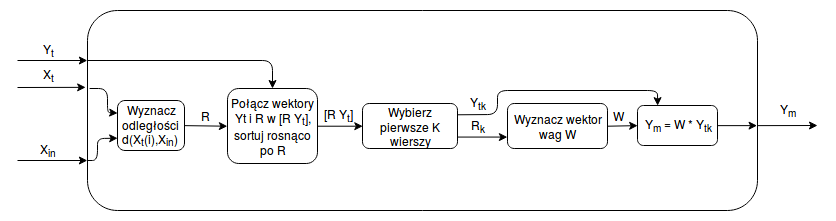
\includegraphics[width=\linewidth]{diagram_knn}
		\caption{Przepływ danych w algorytmie k-NN. Oznaczenia: $X_t$, $Y_t$ - dane uczące; $X_{in}$ - wejście dla którego ma być wyznaczone wyjście modelu; $d(X_t(i)-X_{in}) = ||X_t(i)-X_{in}||_{2} $.}
	\end{figure}
	Metody wyznaczania wag:
	\begin{itemize}
		\item Uśrednianie
		\item Wagi odwrotnie proporcjonalne do odległości
		\item Wagi próbkowane z rozkładu Gaussa w zależności od odległości
	\end{itemize}
\end{frame}

\begin{frame}{Dobór parametrów}
\begin{columns}
	\column{0.5\textwidth}
	\begin{figure}
		\centering
		\makebox[\textwidth][c]{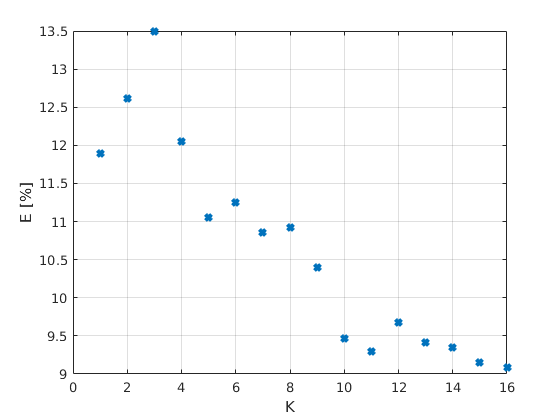
\includegraphics[width=1.2\textwidth]{KNN_dobor_K_1}}
		\caption{Błąd względny dla danych walidacyjnych(1) w zależności od K. Według wykresu najlepszą metodą wyznaczania wartości wyjściowej jest uśrednienie wszystkich danych uczących...}
	\end{figure}
	
	\column{0.5\textwidth}
	\begin{figure}
		\centering
		\makebox[\textwidth][c]{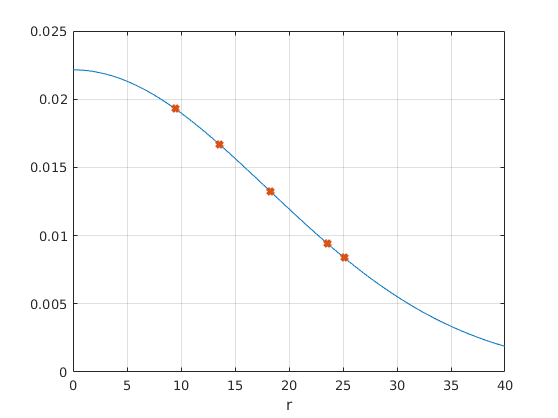
\includegraphics[width=1.2\textwidth]{gauss_weights}}
		\caption{Wagi pośrednie wyznaczane z wykorzystaniem rozkładu Gaussa. Wagi te są normalizowane, aby $\sum_{i}w_i = 1$}
	\end{figure}
\end{columns}
\end{frame}

\begin{frame}{Rezultaty}
$K = 5$, wagi wyznaczane z wykorzystaniem rozkładu Gaussa.
\begin{columns}
	\column{0.5\textwidth}
	\begin{figure}
		\centering
		\makebox[\textwidth][c]{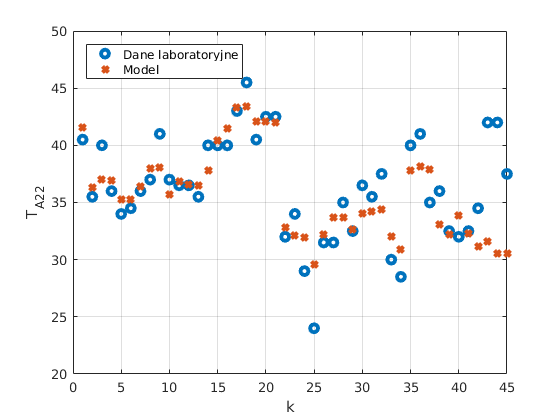
\includegraphics[width=1.2\textwidth]{KNN_daneUczace_1}}
		\caption{Działanie modelu KNN dla danych uczących; $E = 5.62\%$}
	\end{figure}
	
	\column{0.5\textwidth}
	\begin{figure}
		\centering
		\makebox[\textwidth][c]{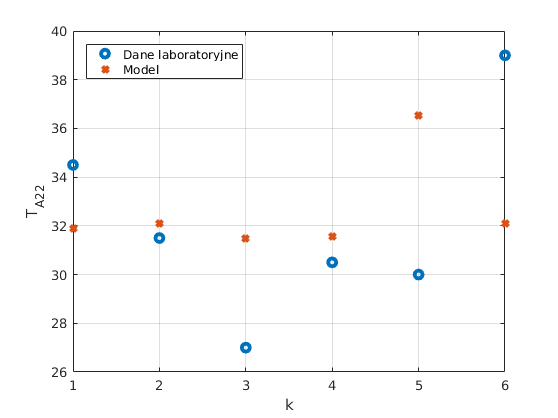
\includegraphics[width=1.2\textwidth]{KNN_daneWalidacyjne_1}}
		\caption{Działanie modelu dla danych walidacyjnych(2); $E = 10.26\%$}
	\end{figure}
\end{columns}
\end{frame}

\begin{frame}{Porównanie modeli, uśrednianie}
\begin{columns}
	\column{0.5\textwidth}
	\begin{figure}
		\centering
		\makebox[\textwidth][c]{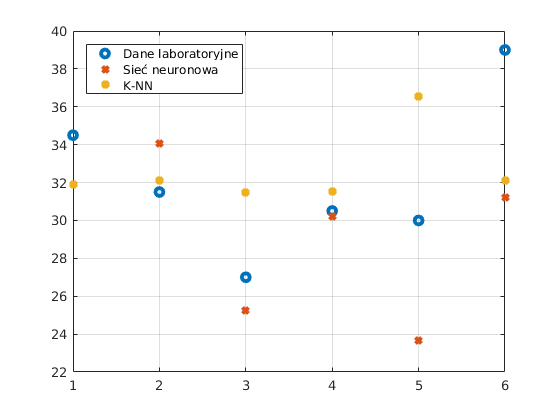
\includegraphics[width=1.2\textwidth]{modele_porownanie}}
		\caption{Porównanie działania modeli dla danych walidacyjnych(2)}
	\end{figure}
	
	\column{0.5\textwidth}
	\begin{figure}
		\centering
		\makebox[\textwidth][c]{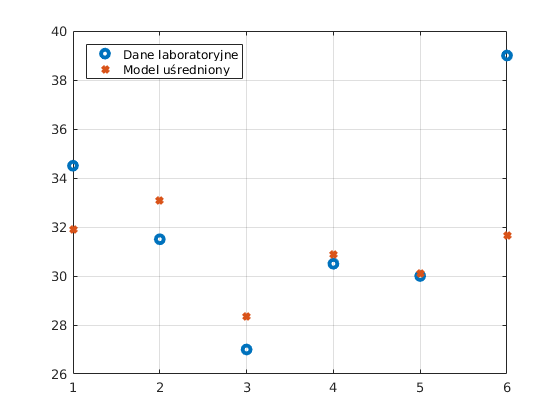
\includegraphics[width=1.2\textwidth]{model_usredniony}}
		\caption{Model uśredniony dla danych walidacyjnych(2); $E = 3.84\%$}
	\end{figure}
\end{columns}
\end{frame}

\end{document}


% przykladowy slajd
%\begin{columns}
%\column{0.5\textwidth}
%\begin{itemize}
%	\item 2 moduły, każdy ma 9 diod
%	\item Prąd pracy modułu: 210mA
%\end{itemize}
%\begin{figure}
%	\includegraphics[width=\linewidth]{rl}
%\end{figure}
%\column{0.5\textwidth}
%\begin{figure}
%	\includegraphics[width=\linewidth]{rl_schematic}
%\end{figure}
%\end{columns}
\grid
